\documentclass[10pt]{article}
\usepackage[margin=1in, paperwidth=8.5in, paperheight=11in]{geometry}
\usepackage{ifpdf, amsmath, amssymb, comment, color, graphicx, stmaryrd, setspace, enumitem, fancyhdr, wrapfig, textcomp, mathptmx, siunitx, multicol}
\usepackage{hyperref}
\hypersetup{
    colorlinks=true,
    urlcolor=blue,
}

\RequirePackage{tikz}
\usetikzlibrary{trees}

\setlength{\headheight}{14.5pt}
\newcommand{\del}{\nabla}
\newcommand{\Q}{\mathbb{Q}}
\newcommand{\R}{\mathbb{R}}
\newcommand{\Z}{\mathbb{Z}}
\newcommand{\vu}{\mathbf{u}}
\newcommand{\vv}{\mathbf{v}}
\newcommand{\vw}{\mathbf{w}}
\newcommand{\vi}{\mathbf{i}}
\newcommand{\vj}{\mathbf{j}}
\newcommand{\vk}{\mathbf{k}}
\newcommand{\vn}{\mathbf{n}}
\newcommand{\vr}{\mathbf{r}}
\newcommand{\vs}{\mathbf{s}}
\newcommand{\va}{\mathbf{a}}
\newcommand{\vF}{\mathbf{F}}
\newcommand{\vL}{\mathbf{L}}
\newcommand{\vT}{\mathbf{T}}
\newcommand{\vN}{\mathbf{N}}
\newcommand{\vB}{\mathbf{B}}
\newcommand{\comp}{\operatorname{comp}}
\newcommand{\proj}{\operatorname{proj}}
\newcommand{\orth}{\operatorname{orth}}
\newcommand\dotp[1][.5]{\,\mathbin{\vcenter{\hbox{\scalebox{#1}{$\bullet$}}}}\,}


\newenvironment{red}{\color{red}}{\ignorespacesafterend}
\newcommand{\blue}[1]{\textcolor{blue}{#1}}
\newcommand{\green}[1]{\textcolor{green}{#1}}
\renewcommand{\section}[1]{\begin{center} \textbf{#1} \\\end{center}}
%
\hyphenpenalty=5000
\setlength{\parindent}{0in}
%\oddsidemargin=-.25in
\allowdisplaybreaks
\pagestyle{fancy}
\renewcommand{\headrulewidth}{0pt}
\lhead{MATH 203}
\rhead{Fall 2024}
%\lfoot{}
%\cfoot{}
\begin{document}
%


%\onehalfspacing
\allowdisplaybreaks
%##################################################################
\section{PS\#6 - Partial derivatives - \red{Answer key} }

\begin{enumerate}[leftmargin=0pt]
\item (\href{https://activecalculus.org/multi/S-10-2-First-Order-Partial-Derivatives.html#A_10_2_2}{Activity 10.2.3}) \begin{red}
    Throughout this solution, constants are in \blue{blue}.
\end{red}
\begin{enumerate}
    \item If $f(x,y) = 3x^3 - 2x^2y^5$, find the partial derivatives $f_x$ and $f_y$.
    \begin{red}
        \begin{align*}
            f_x(x,y) &= \frac{\partial}{\partial x} (3x^3 - 2x^2\blue{y^5} ) &
            f_y(x,y) &= \frac{\partial}{\partial y} (3\blue{x^3} - \blue{2x^2}y^5) \\
            &= 9x^2 - 2(2x)\blue{y^5} &
            &= 0 - \blue{2x^2} (5y^4) \\
            &= 9x^2 - 4xy^5 &
            &= -10x^2 y^4
        \end{align*}
    \end{red}
    \item If $f(x,y) = \displaystyle\frac{xy^2}{x+1}$, find the partial derivatives $f_x$ and $f_y$.
    \begin{red}
        \begin{align*}
            f_x(x,y) &= \frac{\partial}{\partial x} \left( \frac{x\blue{y^2}}{x+1} \right) &
            f_y(x,y) &= \frac{\partial}{\partial y}\left( \blue{\frac{x}{x+1}} y^2 \right) \\
            &= \blue{y^2}\frac{(x+1)(1) - (x)(1)}{(x+1)^2} &
            &= \blue{\frac{x}{x+1}} \cdot 2y \\
            &= \frac{y^2}{(x+1)^2} &
            &= \frac{2xy}{x+1}
        \end{align*}
    \end{red}
    \item If $g(r,s) = rs\cos(r)$, find the partial derivatives $g_r$ and $g_s$.
    \begin{red}
        \begin{align*}
            g_r(r,s) &= \frac{\partial}{\partial r} (\blue{s} r\cos(r)) &
            g_s(r,s) &= \frac{\partial}{\partial s} (\blue{r \cos(r)} s) \\
            &= \blue{s}(r(-\sin(r)) + (1)\cos(r)) &
            &= \blue{r \cos(r)} (1) \\
            &= s\cos(r) - sr\sin(r) &
            &= r\cos(r)
        \end{align*}
    \end{red}
    \item Assuming $f(w,x,y) = (6w+1)\cos(3x^2+4xy^3+y)$, find the partial derivatives $f_w$, $f_x$, and $f_y$.
    \begin{red}
        \begin{align*}
            f_w(w,x,y) &= \frac{\partial}{\partial w} [(6w+1)\blue{\cos(3x^2+4xy^3+y)}] &
            f_x(w,x,y) &= \frac{\partial}{\partial x} [\blue{(6w+1)} \cos(3x^2+4x\blue{y^3}+\blue{y})] \\
            &= (6)\blue{\cos(3x^2+4xy^3+y)} &
            &= \blue{(6w+1)}(-\sin(3x^2+4x\blue{y^3}+\blue{y}))\cdot(6x+4\blue{y^3}) \\
            &= 6\cos(3x^2+4xy^3+y) &
            &= -(6w+1)(6x+4y^3)\sin(3x^2+4xy^3+y) \\
        \end{align*}
        \begin{align*}
            f_y(w,x,y) &= \frac{\partial}{\partial y} [\blue{(6w+1)}\cos(\blue{3x^2}+\blue{4x}y^3+y)] \\
            &= \blue{(6w+1)}(-\sin(\blue{3x^2}+\blue{4x}y^3+y))\cdot(\blue{4x}\cdot 3y^2 + 1) \\
            &= -(6w+1)(12xy^2+1)\sin(3x^2+4xy^3+y)
        \end{align*}
    \end{red}
    \item Find all possible first-order partial derivatives of $q(x,t,z) =
    \displaystyle \frac{x2^tz^3}{1+x^2}$.
    \begin{red}
        \begin{align*}
            q_x(x,t,z) &= \frac{\partial}{\partial x}\left(\blue{2^tz^3}\frac{x}{1+x^2}\right) &
            q_t(x,t,z) &= \frac{\partial}{\partial t}\left(\blue{\frac{xz^3}{1+x^2}}2^t\right) &
            q_z(x,t,z) &= \frac{\partial}{\partial z}\left(\blue{\frac{x2^t}{1+x^2}}z^3\right) \\
            &= \blue{2^tz^3}\frac{(1+x^2)(1) - (x)(2x)}{(1+x^2)^2} &
            &= \blue{\frac{xz^3}{1+x^2}}(2^t\ln(2)) &
            &= \blue{\frac{x2^t}{1+x^2}}(3z^2) \\
            &= \frac{2^t z^3 (1-x^2)}{(1+x^2)^2} &
            &= \frac{x z^3 2^t \ln(2)}{1+x^2} &
            &= \frac{3x 2^t z^2}{1+x^2}
        \end{align*}
    \end{red}
\end{enumerate}

\item (\href{https://activecalculus.org/multi/S-10-2-First-Order-Partial-Derivatives.html#A_10_2_11}{Activity 10.2.4}) The speed of sound $C$ traveling through ocean water is a function of temperature, salinity and depth. It may be modeled by the function
\begin{equation*}
C(T,S, D)=1449.2+4.6T-0.055T^2+0.00029T^3+(1.34-0.01T)(S-35)+0.016D.
\end{equation*}
Here $C$ is the speed of sound in meters/second, $T$ is the temperature in degrees Celsius, $S$ is the salinity in grams/liter of water, and $D$ is the depth below the ocean surface in meters.
\begin{enumerate}
    \item State the units in which each of the partial derivatives, $C_T$, $C_S$, and $C_D$, are expressed and explain the physical meaning of each.
    
    \begin{red}
    $C_T$ is measured in $\dfrac{\textrm{m/s}}{^\circ C}$, and it tells us how much the speed of sound in water changes as the temperature changes.
    
    $C_S$ is measured in $\dfrac{\textrm{m/s}}{\textrm{gm/L}}$, and it tells us how much the speed of sound in water changes as the salinity changes.
    
    $C_D$ is measured in $\dfrac{\textrm{m/s}}{\textrm{m}}$, and it tells us how much the speed of sound in water changes as the depth changes.
    \end{red}
    \item Find the partial derivatives $C_T$, $C_S$, and $C_D$. 
    
    \begin{red}
    \[C_T(T,S, D) = 4.6 - 0.11 T + 0.00087 T^2 -0.01(S-35) \]
    \[C_S(T,S, D) = 1.34-0.01T \]
    \[C_D(T,S, D) = 0.016\]
    \end{red}
    \item Evaluate each of the three partial derivatives at the point where $T=10$, $S=35$ and $D=100$. What does the sign of each partial derivative tell us about the behavior of the function $C$ at the point $(10, 35, 100)$?
    
    \begin{red}
    $C_T(10, 35, 100) = 3.587$ -- so the speed of sound \textbf{increases} as the temperature goes up from this point.
    
    $C_S(10, 35, 100) = 1.24$ -- so the speed of sound \textbf{increases} as the salinity goes up from this point.
    
    $C_D(10, 35, 100) = 0.016$ -- so the speed of sound \textbf{increases} as the depth increases from this point.
    \end{red}
\end{enumerate}
\item (\href{https://activecalculus.org/multi/S-10-2-First-Order-Partial-Derivatives.html#A_10_2_12}{Activity 10.2.5}) The wind chill, as frequently reported, is a measure of how cold it feels outside when the wind is blowing. In the table below, the wind chill $w$, measured in degrees Fahrenheit, is a function of the wind speed $v$, measured in miles per hour, and the ambient air temperature $T$, also measured in degrees Fahrenheit. We thus view $w$ as being of the form $w=w(v,T).$
\[\begin{array}{rrrrrrrrrrrr}
\hline v \backslash T & -30 & -25 & -20 & -15 & -10 & -5 & 0 & 5 & 10 & 15 & 20 \\
\hline 5 & -46 & -40 & -34 & -28 & -22 & -16 & -11 & -5 & 1 & 7 & 13 \\
\hline 10 & -53 & -47 & -41 & -35 & -28 & -22 & -16 & -10 & -4 & 3 & 9 \\
\hline 15 & -58 & -51 & -45 & -39 & -32 & -26 & -19 & -13 & -7 & 0 & 6 \\
\hline 20 & -61 & -55 & -48 & -42 & -35 & -29 & -22 & -15 & -9 & -2 & 4 \\
\hline 25 & -64 & -58 & -51 & -44 & -37 & -31 & -24 & -17 & -11 & -4 & 3 \\
\hline 30 & -67 & -60 & -53 & -46 & -39 & -33 & -26 & -19 & -12 & -5 & 1 \\
\hline 35 & -69 & -62 & -55 & -48 & -41 & -34 & -27 & -21 & -14 & -7 & 0 \\
\hline 40 & -71 & -64 & -57 & -50 & -43 & -36 & -29 & -22 & -15 & -8 & -1 \\
\hline
\end{array}\]
\begin{enumerate}
    \item Estimate the partial derivative $w_v(20,-10)$. What are the units on this quantity and what does it mean?
    
    \begin{red}
    \begin{align*}
        w_v(20, -10) &\approx \frac{w(25, -10) - w(15, -10)}{25-15} = \frac{-37 - (-32)}{10} = \frac{-5}{10} = -0.5 \frac{^\circ \textrm{F}}{\textrm{mph}}.
    \end{align*}
    That is, if the windspeed goes up by 1 mph, the perceived temperature will drop by $0.5^\circ$ F.
    \end{red}
    
    \item Estimate the partial derivative $w_T(20,-10)$. What are the units on this quantity and what does it mean?
    \begin{red}
    \begin{align*}
        w_T(20,-10) &\approx 
        \frac{w(20, -5) - w(20,-15)}{-5 - (-15)} = 
        \frac{-29-(-42)}{10} = \frac{13}{10} = 1.3 \frac{^\circ \textrm{F}}{^\circ\textrm{F}}.
    \end{align*}
    That is, if the ambient temperature goes up by $1^\circ$ F, the perceived temperature will go up by $1.3^\circ$ F.
    \end{red}
    
    \item Use your results to estimate the wind chill $w(18, -10)$.
    
    \begin{red}
    The windspeed has gone down by 2 mph. Each 1 mph decrease in windspeed causes an $0.5^\circ$ F \textbf{increase} in perceived temperature. Therefore, $w(18, -10)$ should be about $1^\circ$ F warmer than $w(20, -10),$ which is $-35$, so it should be $-34^\circ$ F.
    
    In symbols: 
    \begin{align*}
        w(18, -10) &\approx w(20, -10) + (18-20) \cdot w_v(20, -10) \\
        &= -35^\circ \textrm{F} + (-2\textrm{ mph})\cdot \left(-0.5 \frac{^\circ \textrm{F}}{\textrm{mph}}\right) \\
        &= -35^\circ \textrm{F} + 1^\circ \textrm{F} = -34^\circ \textrm{F}.
    \end{align*}
    \end{red}
    
    \item Use your results to estimate the wind chill $w(20, -12)$.
    
    \begin{red}
    The ambient temperature has dropped by 2 degrees. Each 1 degree decrease in ambient temperature causes a 1.3 degree decrease in perceived temperature. Therefore, $w(20, -12)$ should be about $2.6$ degrees colder than $w(20, -10)$, which is $-35^\circ$ F, so it should be $-37.6^\circ$ F.
    
    In symbols: 
    \begin{align*}
        w(20, -12) &\approx w(20, -10) + (-12-(-10)) \cdot w_T(20, -10) \\
        &= -35^\circ \textrm{F} + (-2^\circ\textrm{F})\cdot \left(1.3 \frac{^\circ \textrm{F}}{^\circ \textrm{F}}\right) \\
        &= -35^\circ \textrm{F} -2.6^\circ \textrm{F} = -37.6^\circ \textrm{F}.
    \end{align*}
    \end{red}
    
    \item Consider how you might combine your previous results to estimate the wind chill $w(18, -12)$. Explain your process.
    
    \begin{red}
    From the original $-35^\circ$F, the perceived temperature should go up by 1 (from the decrease in windspeed) and down by 2.6 (from the decrease in temperature). So I bet $w(18, -12) \approx -35 + 1 - 2.6 -36.6^\circ$F.
    \end{red}
\end{enumerate}
\item (\href{https://activecalculus.org/multi/S-10-2-First-Order-Partial-Derivatives.html#A_10_2_13}{Activity 10.2.6}) Shown in the figure below is a contour plot of a function $f$. The values of the function on a few of the contours are indicated to the left of the figure.
\begin{center}
    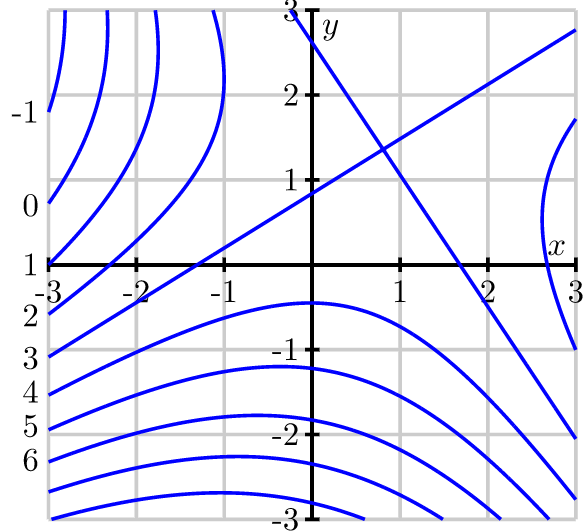
\includegraphics[width=0.5\textwidth]{../images/10-2-6.png}
\end{center}
\begin{enumerate}
    \item Estimate the partial derivative $f_x(-2, -1).$
    
    \begin{red}
    We can use the contours to read off some approximate values and use a symmetric difference. 
    
    \textbf{NOTE:} I'm using a step size of 1 -- your answer may be a little different from this if you chose a different step size. Same deal in parts (b) and (c).
    \begin{align*}
        f(-3, -1) &\approx 3 \\
        f(-1, -1) &\approx 4.5 \\
        f_x(-2,-1) &\approx 
        \frac{f(-1, -1)-f(-3, -1)}{-1-(-3)} \\
        &= \frac{4.5-3}{2} = 0.75
    \end{align*}
    \end{red}
    
    \item Estimate the partial derivative $f_y(-2, -1).$
    
    \begin{red}
    Same game -- we can use the contours to read off some approximate values and use a symmetric difference: 
    \begin{align*}
        f(-2, -2) &\approx 6 \\
        f(-2, 0) &\approx 2.5 \\
        f_y(-2,-1) &\approx 
        \frac{f(-2, 0) - f(-2, -2)}{0-(-2)} \\
        &= \frac{2.5-6}{2} = -1.75
    \end{align*}
    \end{red}
    
    \item Estimate the partial derivatives $f_x(-1, 2)$ and $f_y(-1, 2)$.
    \begin{red}
    \begin{multicols}{2}
    \begin{align*}
        f(0, 2) &\approx 2.5\\
        f(-2, 2) &\approx 0.5 \\
        f_x(-1,2) &\approx 
        \frac{f(0,2)-f(-2,2)}{0-(-2)} \\
        &= \frac{2.5-0.5}{2} = 1
    \end{align*}
    
    \begin{align*}
        f(-1,1) &\approx 2.5 \\
        f(-1,3) &\approx 2.5 \\
        f_y(-1,2) &\approx
        \frac{f(-1,3)-f(-1,1)}{3-1} \\
        &= \frac{2.5-2.5}{2} = 0
    \end{align*}
    \end{multicols}
    \end{red}
    
    \item Locate, if possible, one point $(x,y)$ where $f_x(x,y)=0$.
    
    \begin{red}
    Looks like at about $(0, -0.5)$, if I move in the $x$ direction, the heights on the contour map don't change much.
    \end{red}
    
    \item Locate, if possible, one point $(x,y)$ where $f_x(x,y)<0$.
    
    \begin{red}
    Looks like at about $(1,-2)$, if I move in the $x$ direction, I'm going downhill.
    \end{red}
    
    \item Locate, if possible, one point $(x,y)$ where $f_y(x,y)>0$.
    
    \begin{red}
    Looks like at about $(1,2)$, if I move in the $y$ direction, I'm going (very slightly) uphill.
    
    \textbf{NOTE:} Of course there are other points that will work for all three of these parts.
    \end{red}

\end{enumerate}

\item (\href{https://activecalculus.org/multi/S-10-2-First-Order-Partial-Derivatives.html#Ez_10_2_1_5}{AC Multi 10.2 Exercise 14}) Let $f(x, y) = \tfrac{1}{2}xy^2$ represent the kinetic energy in Joules of an object of mass $x$ in kilograms with velocity $y$ in meters per second. Let $(a, b)$ be the point $(4,5)$ in the domain of $f$.
    \begin{enumerate}
        \item Calculate $f_x(a,b)$.
        
        \begin{red}
            First of all, let's calculate $f_x(x,y).$ Holding $y$ constant, we'll take the derivative with respect to $x$:
            \[f_x(x,y) = \tfrac{1}{2}y^2.\]
            Now we'll evaluate this at our point: $f_x(a, b) = f_x(4, 5) = \tfrac{1}{2}\cdot 5^2 = \tfrac{25}{2}.$
            (By the way, the units on this quantity are Joules per kilogram.)
        \end{red}
        \item Explain as best you can in the context of kinetic energy what the partial derivative
        \[f_{x}(a, b)=\lim _{h \rightarrow 0} \frac{f(a+h, b)-f(a, b)}{h}\]
        tells us about kinetic energy.
        
        \begin{red}
            This essentially tells us how much the kinetic energy changes per unit change in \textbf{mass} of the object. 
            
            Dimensional analysis helps: Note here since $h$ is being added to the $x$ term, it's a small change in \textbf{mass}. Thus, since the numerator has the same output as $f$, it's Joules; since the denominator is an $h$, it's kilograms. So, the units on this quantity are Joules per kilogram.
        \end{red}
        
        \item Calculate $f_y(a,b)$.
        
        \begin{red}
            First of all, let's calculate $f_y(x,y).$ Holding $x$ constant, we'll take the derivative with respect to $y$:
            \[f_y(x,y) = \tfrac{1}{2}x\cdot 2y = xy.\]
            Now we'll evaluate this at our point: $f_y(a, b) = f_y(4, 5) = 4 \cdot 5 = 20.$
            (By the way, the units on this quantity are Joules per (meters per second).)
            
            
        \end{red}
        
        \item Explain as best you can in the context of kinetic energy what the partial derivative
        \[f_{y}(a, b)=\lim _{h \rightarrow 0} \frac{f(a, b+h)-f(a, b)}{h}\]
        tells us about kinetic energy.
        
        \begin{red}
            This essentially tells us how much the kinetic energy changes per unit change in \textbf{velocity} of the object. 
            
            Dimensional analysis helps: Note here since $h$ is being added to the $y$ term, it's a small change in \textbf{velocity}. Thus, since the numerator has the same output as $f$, it's Joules; since the denominator is an $h$, it's meters per second. So, the units on this quantity are Joules per (meters per second).
        \end{red}
        
        \item Often we are given certain graphical information about a function instead of a rule. We can use that information to approximate partial derivatives. For example, suppose that we are given a contour plot of the kinetic energy function (as in the figure below) instead of a formula. Use this contour plot to approximate $f_x(4, 5)$ and $f_y(4, 5)$ as best you can. Compare to your calculations from earlier parts of this exercise.
        
        \begin{center}
            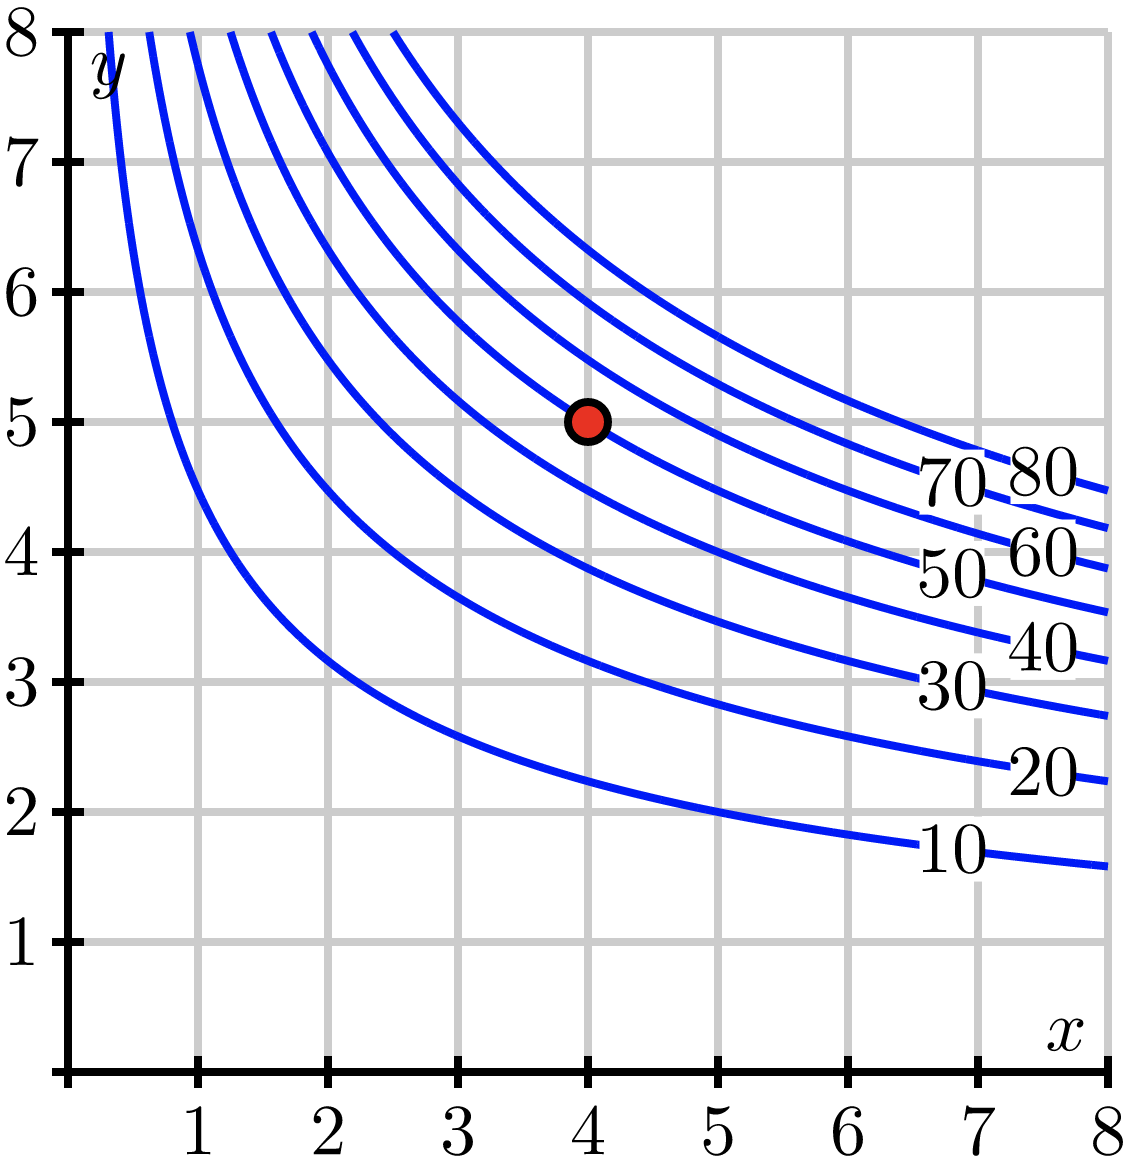
\includegraphics[width=0.5\textwidth]{../images/10-2-14.png}
        \end{center}
        
        \begin{red}
            To find $f_x(4,5)$: I'm going to stand at the point $(4,5)$ and, holding $y$ constant, take a small step in the $x$ direction, and see what happens to my output values.
            
            When I'm on the point $(4,5)$, I'm on the $z = 50$ contour, so I know that $f(4,5) = 50$. If I take a little step in the $x$ direction, I land just a little above the $z = 60$ contour, so I know that $f(4+1, 5) \approx 60$ or $62$ish. Therefore, my step of 1 kg has produced a change of 10 or 12 Joules, so $f_x(4,5) \approx 10/1$ or $12/1$ Joules per kg. This is pretty close to the value we calculated earlier, $\tfrac{25}{2} = 12.5$.
            
            To find $f_y(4,5)$: I'm going to stand at the point $(4,5)$ and, holding $x$ constant, take a small step in the $y$ direction, and see what happens to my output values.
            
            When I'm on the point $(4,5)$, I'm on the $z = 50$ contour, so I know that $f(4,5) = 50$. If I take a little step in the $y$ direction, I land just a little above the $z = 70$ contour, so I know that $f(4, 5+1) \approx 70$ or $72$ish. Therefore, my step of 1 m/s has produced a change of 20 or 22 Joules, so $f_y(4,5) \approx 20/1$ or $22/1$ Joules per m/s. This is pretty close to the value we calculated earlier, $20$.
            
            
        \end{red}
    \end{enumerate}

\end{enumerate}


\end{document}